\documentclass[12pt]{article}
\usepackage{amsmath}
\usepackage{amssymb}
\usepackage[letterpaper,margin=0.85in,centering]{geometry}
\usepackage{fancyhdr}
\usepackage{enumerate}
\usepackage{lastpage}
\usepackage{multicol}
\usepackage{graphicx}
\usepackage{polynom}
\usepackage{tikz}
\usetikzlibrary{calc, positioning, decorations.pathmorphing}

\reversemarginpar

\pagestyle{fancy}
\cfoot{Page \thepage \ of \pageref{LastPage}}\rfoot{{\bf Total Points: 40}}
\chead{MATH 1010A}\lhead{Test \# 2}\rhead{Monday, 16\textsuperscript{th} November, 2015}

\newcommand{\points}[1]{\marginpar{\hspace{24pt}[#1]}}
\newcommand{\skipline}{\vspace{12pt}}
%\renewcommand{\headrulewidth}{0in}
\headheight 30pt

\newcommand{\di}{\displaystyle}
\newcommand{\R}{\mathbb{R}}
\newcommand{\aaa}{\mathbf{a}}
\newcommand{\bbb}{\mathbf{b}}
\newcommand{\ccc}{\mathbf{c}}
\newcommand{\dotp}{\boldsymbol{\cdot}}
\newcommand{\abs}[1]{\lvert #1\rvert}
\newcommand{\len}[1]{\lVert #1\rVert}
\newcommand{\ivec}{\,\boldsymbol{\hat{\imath}}}
\newcommand{\jvec}{\,\boldsymbol{\hat{\jmath}}}
\newcommand{\kvec}{\,\boldsymbol{\hat{k}}}
\DeclareMathOperator{\comp}{comp}

\begin{document}

\author{Instructor: Sean Fitzpatrick}
\thispagestyle{plain}
\begin{center}
\emph{University of Lethbridge}\\
Department of Mathematics and Computer Science\\
16\textsuperscript{th} November, 2015, 4:00 - 4:50 pm\\
{\bf MATH 1010A - Test \#2}\\
\end{center}
\skipline \skipline \skipline \noindent \skipline
Last Name:\underline{\hspace{50pt}{\bf Solutions}\hspace{248pt}}\\
\skipline
First Name:\underline{\hspace{50pt}{\bf The}\hspace{275pt}}\\
\skipline
Student Number:\underline{\hspace{323pt}}\\
\skipline
Tutorial Section: \underline{\hspace{320pt}}\\


\vspace{0.5in}


\begin{quote}
 {\bf Record your answers below each question in the space provided.    Left-hand pages may be used as scrap paper for rough work.  If you want any work on the left-hand pages to be graded, please indicate so on the right-hand page.
 
 \bigskip
 
Partial credit will be awarded for partially correct work, so be sure to show your work, and include all necessary justifications needed to support your arguments.

\bigskip

No external aids are allowed, with the exception of a 5-function calculator.}
\end{quote}


\vspace{0.5in}

For grader's use only:

\begin{table}[hbt]
\begin{center}
\begin{tabular}{|l|r|} \hline
Problem &Grade\\
\hline \hline
\cline{1-2} 1 & \enspace\enspace\enspace\enspace\enspace\enspace/8\\
\cline{1-2} 2 & \enspace\enspace\enspace\enspace\enspace\enspace/12\\
\cline{1-2} 4 & \enspace\enspace\enspace\enspace\enspace\enspace/10\\
\cline{1-2} 5 & \enspace\enspace\enspace\enspace\enspace\enspace/10\\
\cline{1-2} Total & \enspace\enspace\enspace\enspace\enspace\enspace/40\\
\hline
\end{tabular}

\skipline

\skipline

\skipline

A
\end{center}
\end{table}
\newpage


\begin{enumerate}
\item Match the following functions with their graphs below: \points{8}
\begin{align*}
 f(x) &= \dfrac{1}{2}(x+1)(x-1)(x-2)^2, &h(x) &= \dfrac{x^2}{x^2-1},\\
 g(x) &= x^2(x+2)^2(1-x), &k(x) &= \dfrac{x-3}{x(x+2)}
\end{align*}

\bigskip

\begin{multicols}{2}
 \begin{center}
  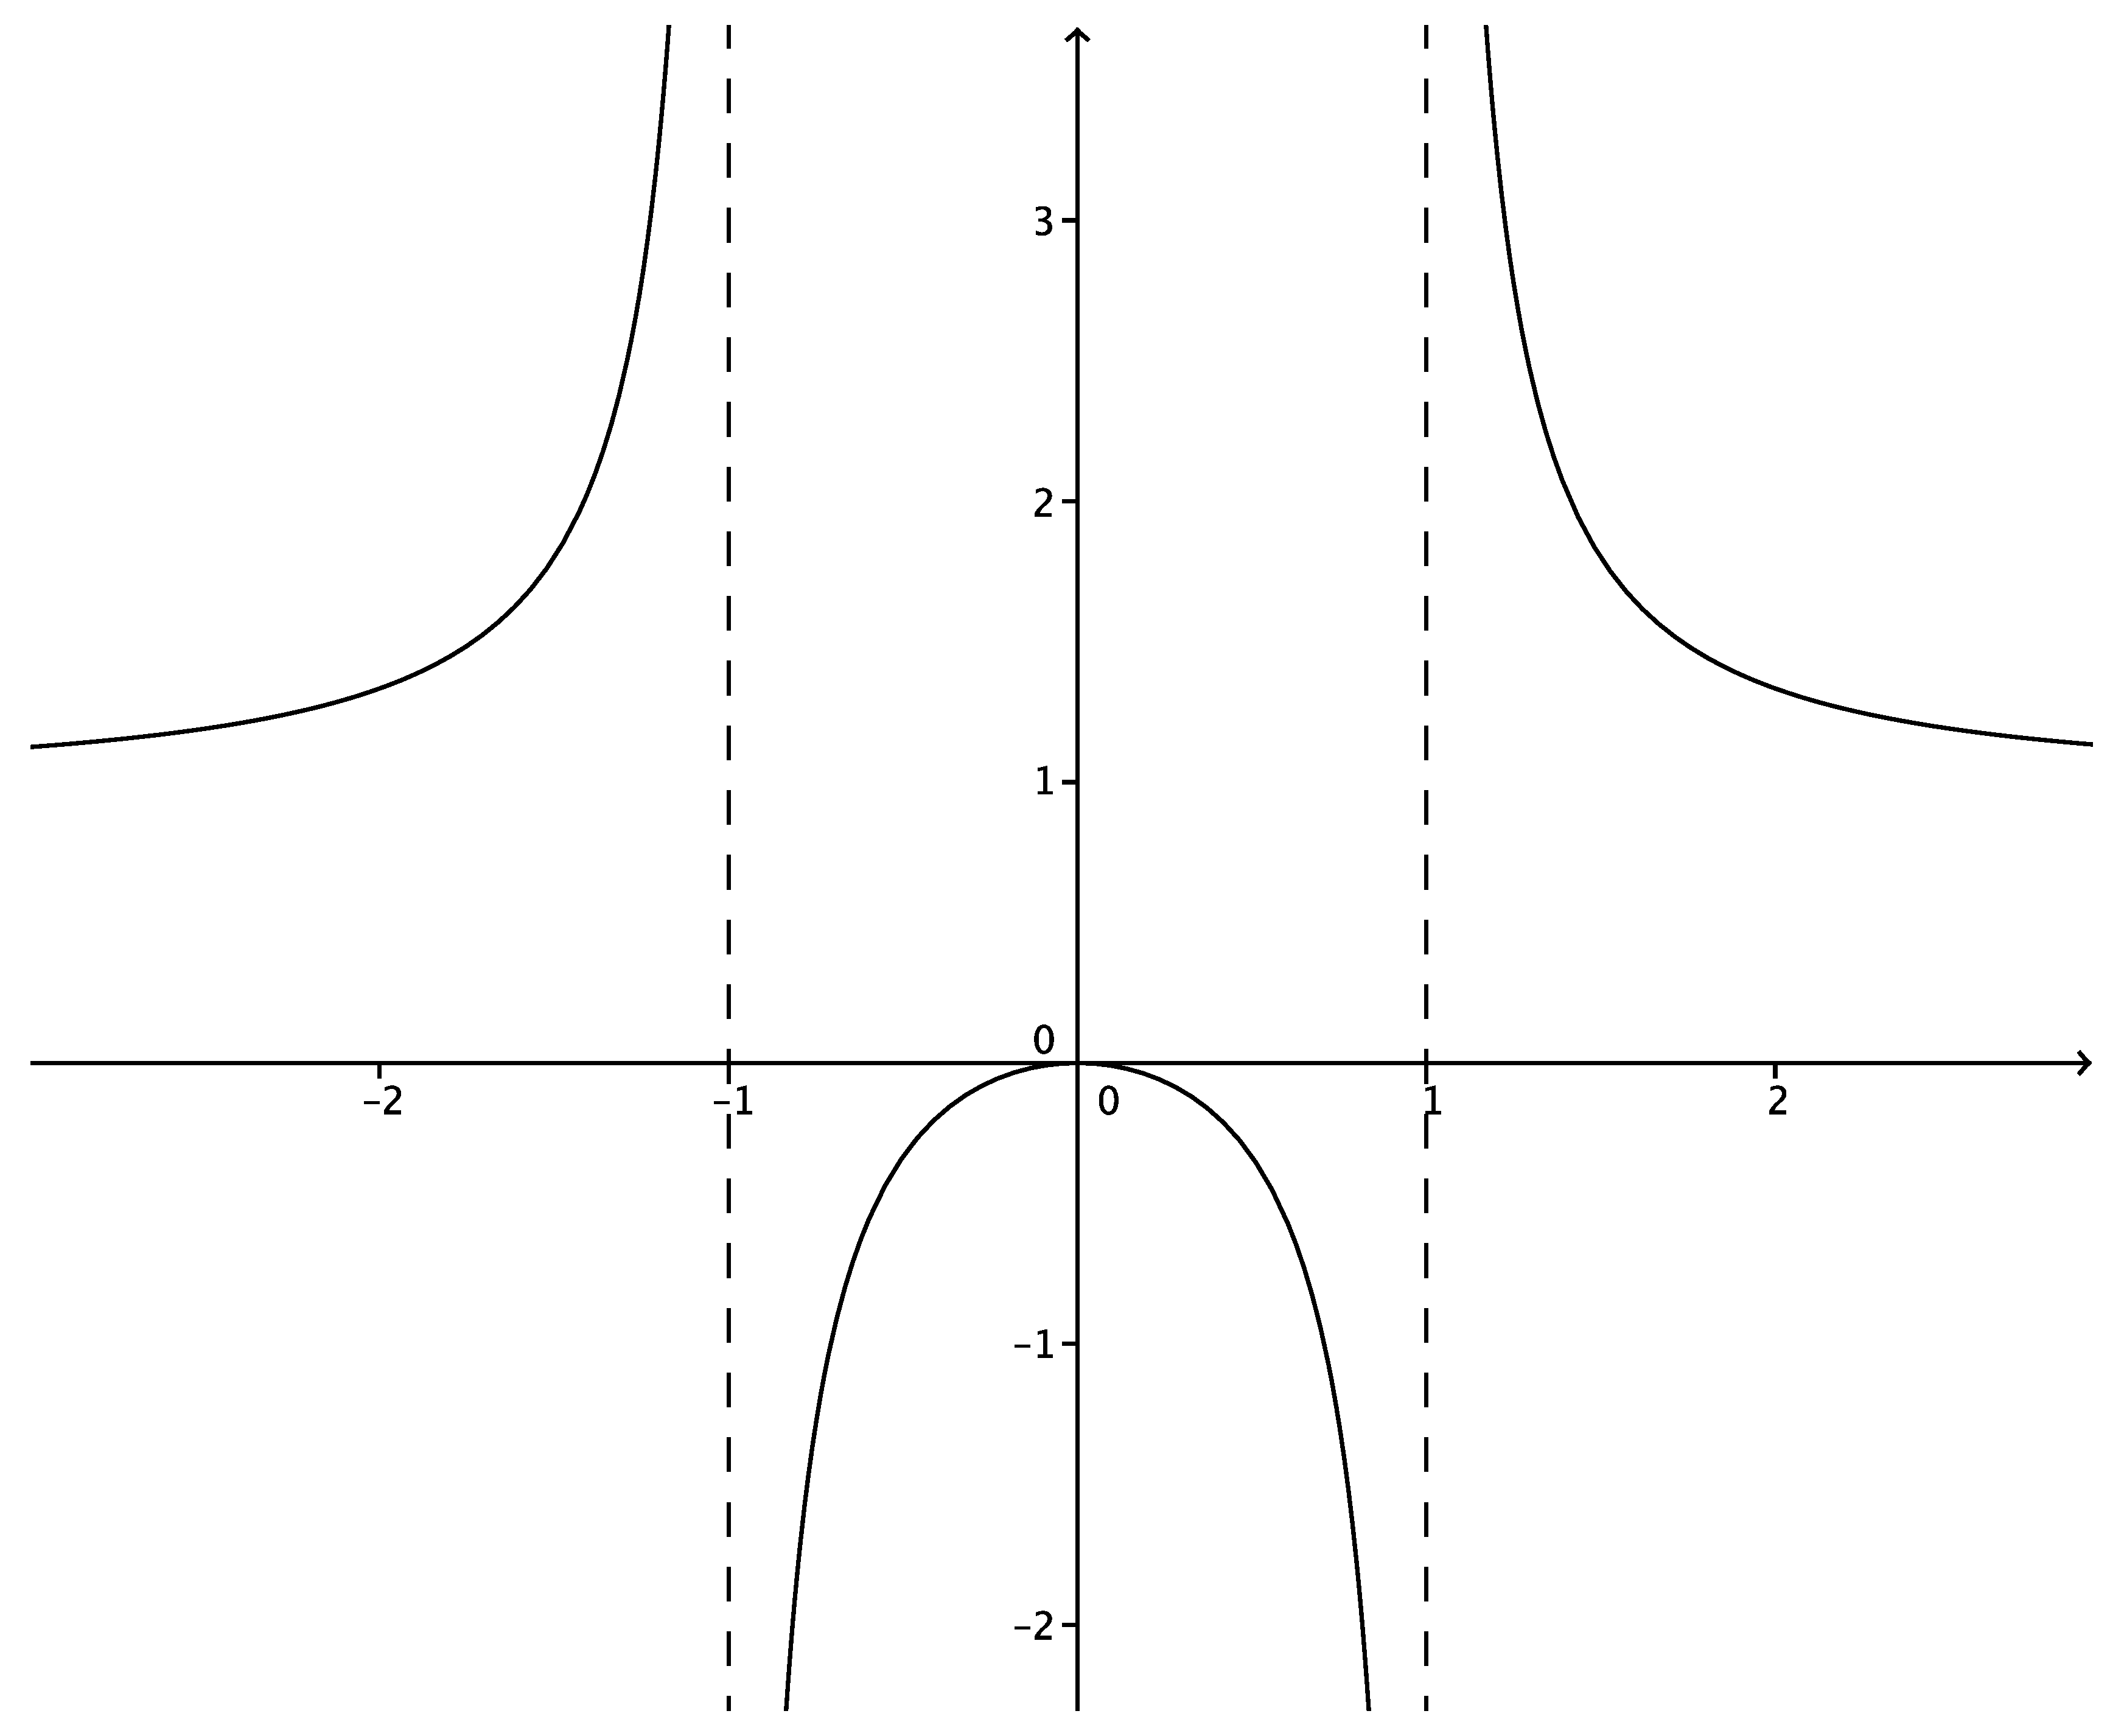
\includegraphics[width=3.25in]{rat1(b)}

$h(x)$
 \end{center}

\bigskip

\bigskip

 \begin{center}
   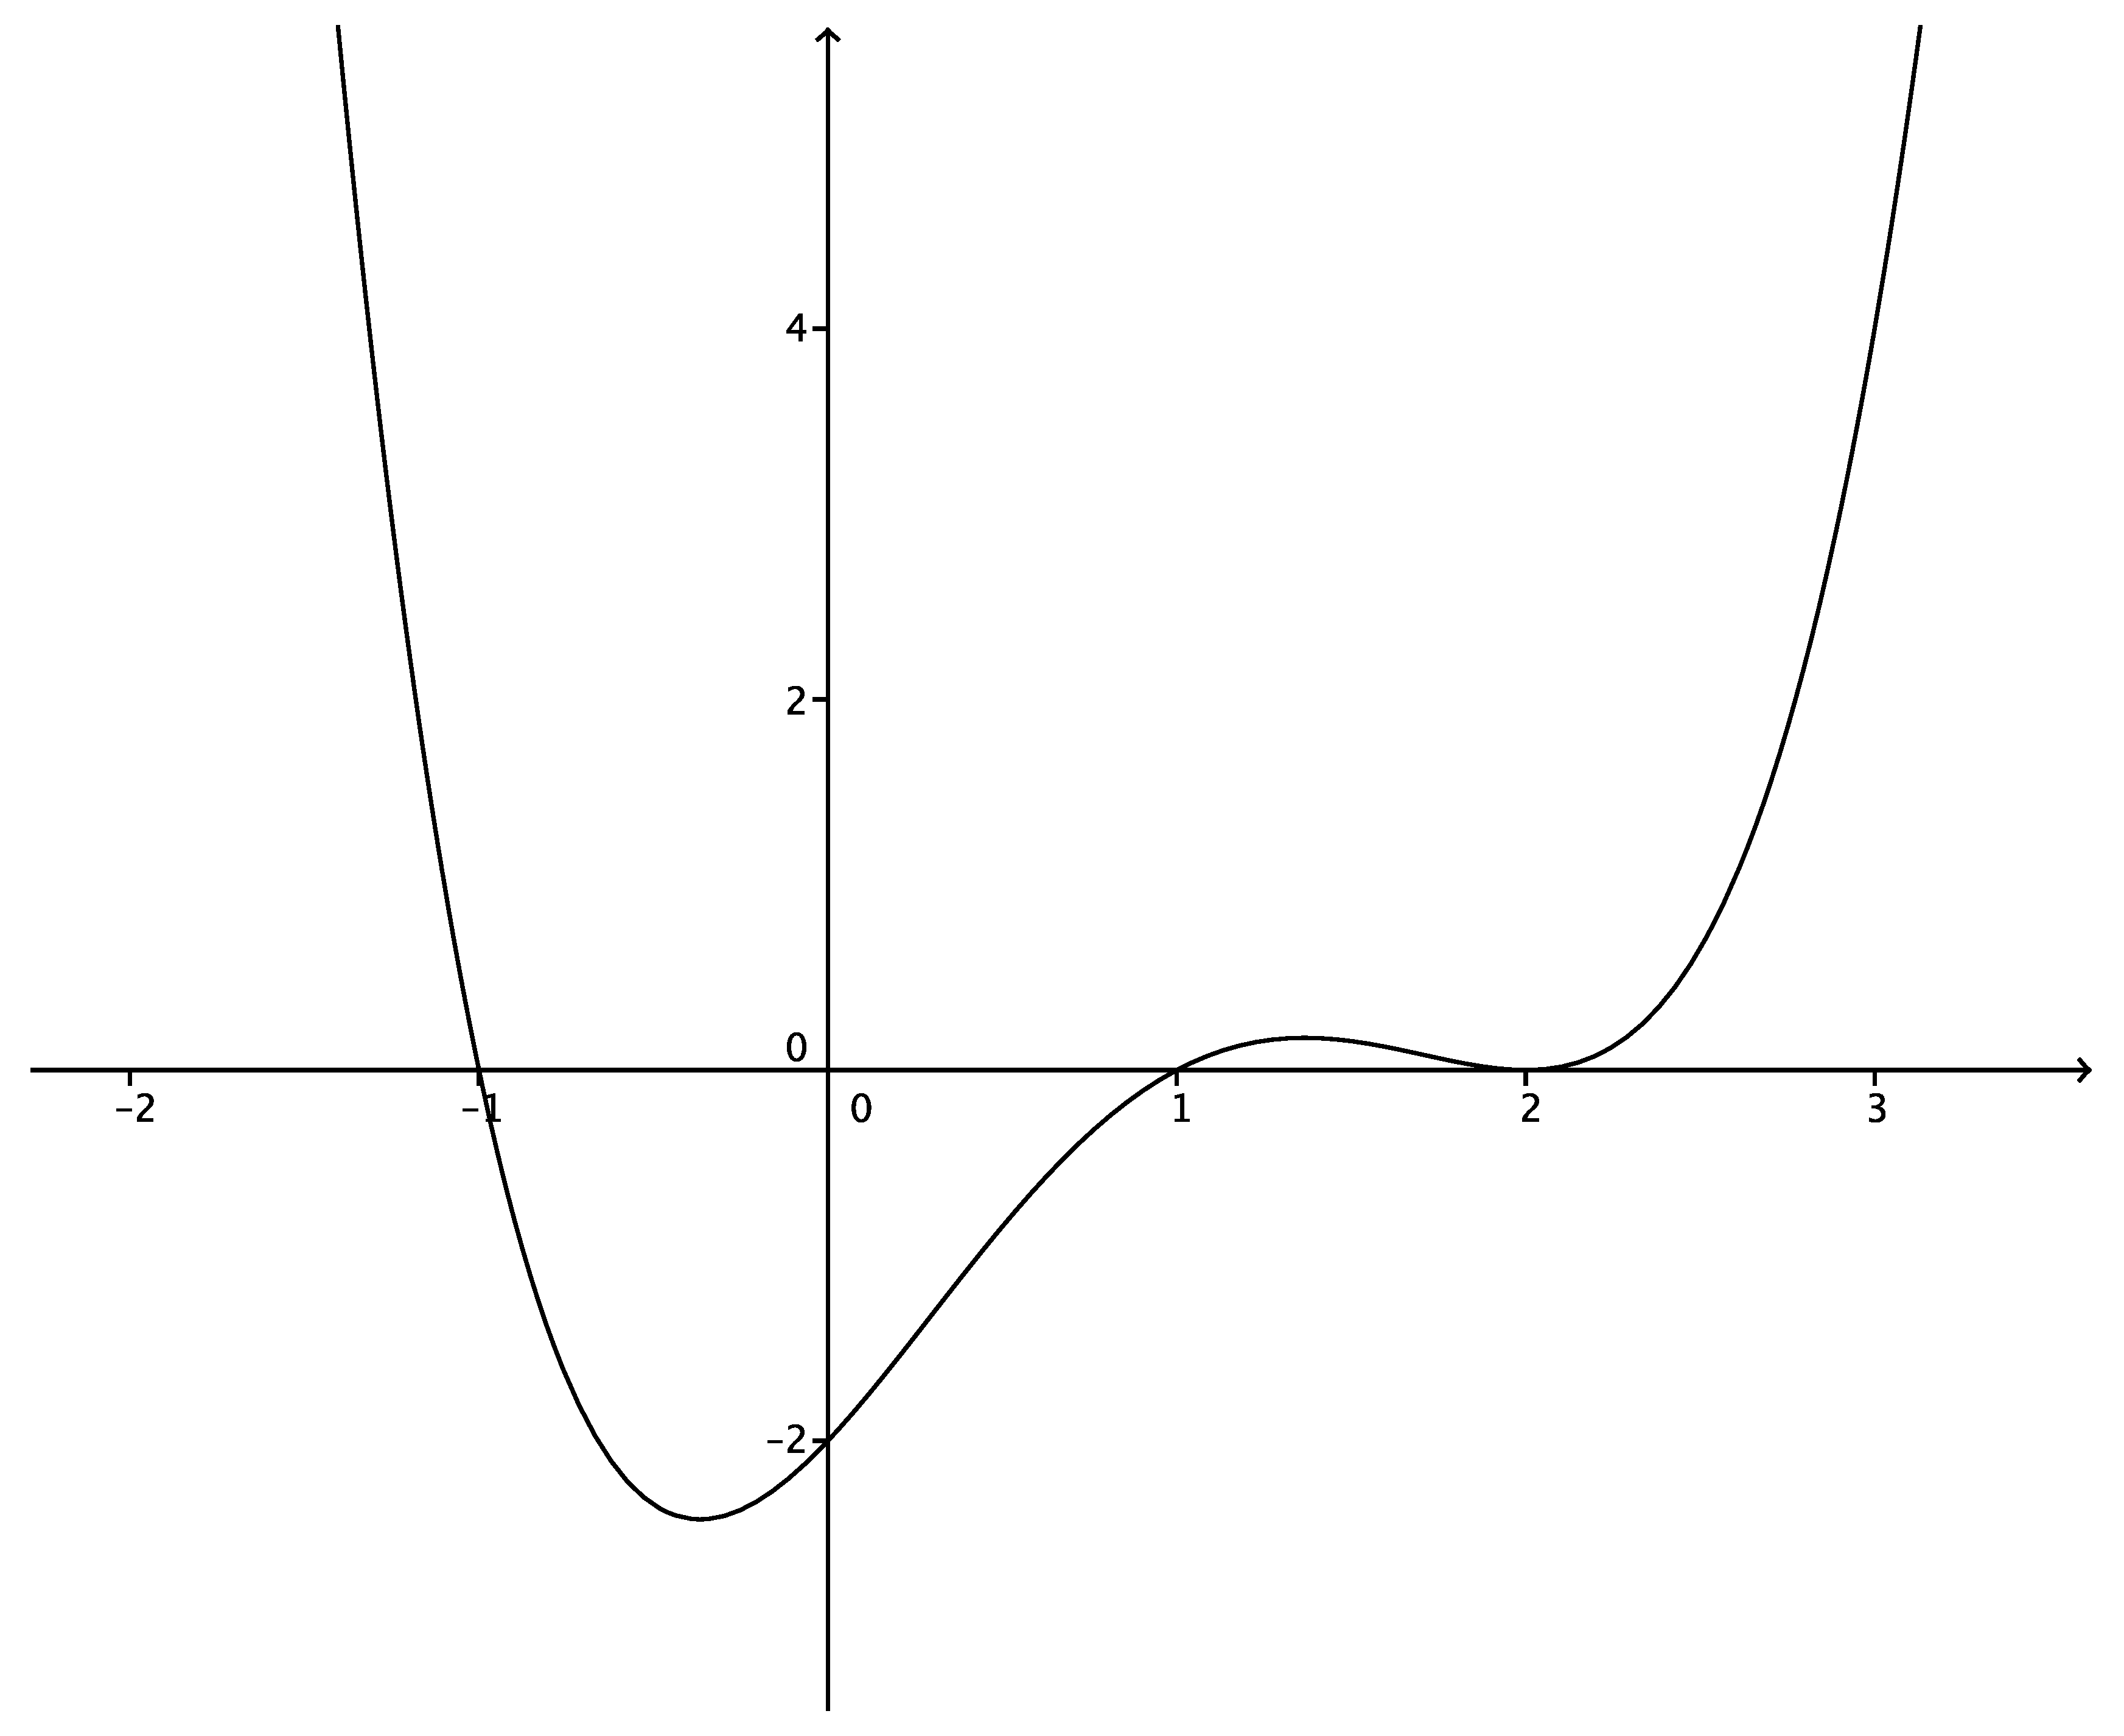
\includegraphics[width=3.25in]{poly1(a)}

$f(x)$
 \end{center}
 \begin{center}
   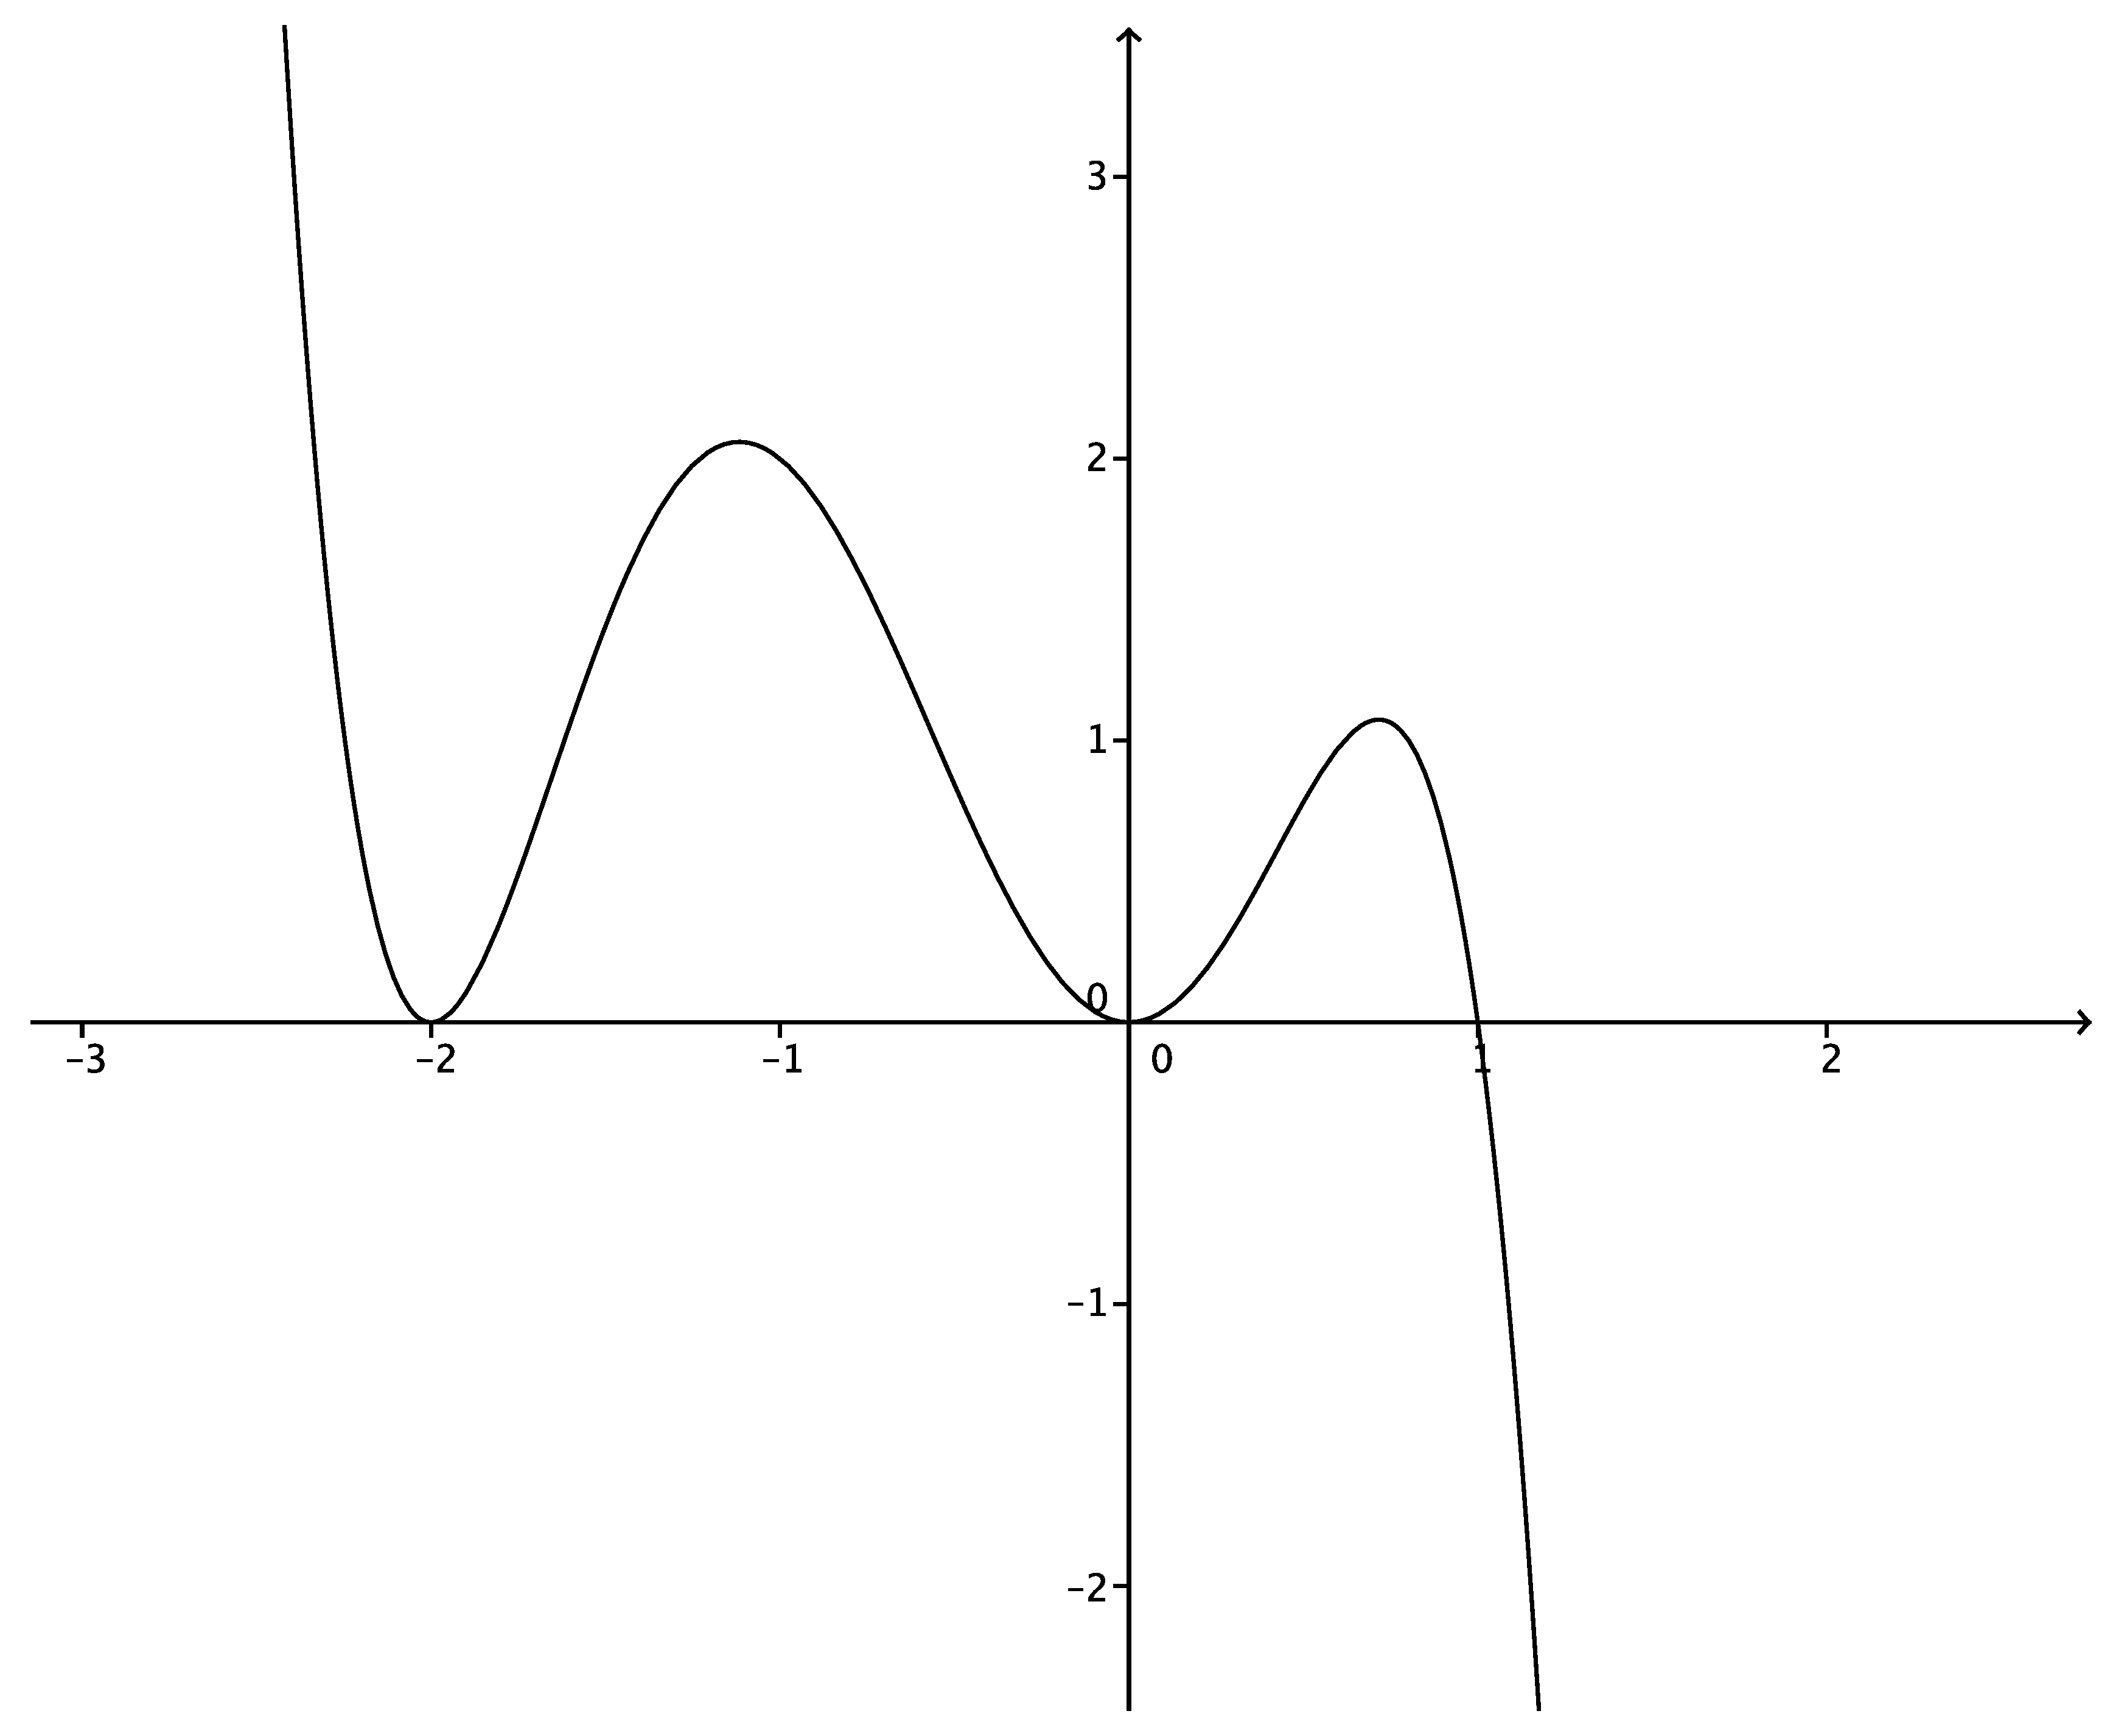
\includegraphics[width=3.25in]{poly1(c)}

$g(x)$
 \end{center}

\bigskip

\bigskip

 \begin{center}
   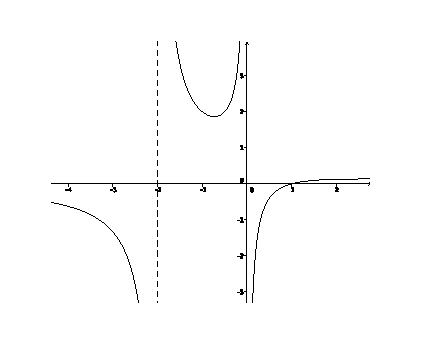
\includegraphics[width=3.25in]{rat1(c)}

$k(x)$
 \end{center}
\end{multicols}


\newpage

\item Let $f(x) = x^3+2x^2-5x-6$.
\begin{enumerate}
 \item Show that $x+1$ is a factor of $f(x)$. \points{1}

\bigskip

Since $f(-1) = (-1)^3+2(-1)^2-5(-1)-6 = -1+2+5-6 = 0$, we know that $x+1$ is a factor of $f(x)$, by the Factor Theorem.

\bigskip

 \item Find $a,b\in\R$ such that $f(x) = (x+1)(x-a)(x-b)$. \points{4}

\bigskip

From (a), we know that $f(x)=(x+1)g(x)$ for some quadratic function $g(x)$. We can find $g(x)$ using long division, as follows:
\[
 \polylongdiv{x^3+2x^2-5x-6}{x+1}
\]
It follows that $f(x) = (x+1)(x^2+x-6) = (x+1)(x+3)(x-2)$, so we can take $a=-3$ and $b=2$.

\bigskip

 \item Construct the sign diagram for $f(x)$.  \points{2}

\bigskip

From part (b), we see that $f$ changes sign at $x=2$, $x=-1$, and $x=-3$. Since $f(x)>0$ for $x>2$, we obtain:
\begin{center}
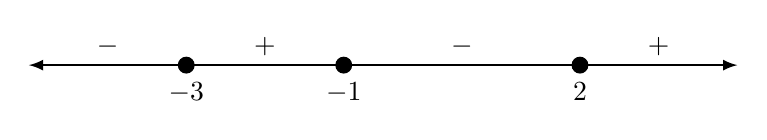
\begin{tikzpicture}[>=latex]
  \draw [thick, <->] (-5,0) -- (4,0);
  \draw [fill] (-3,0) circle [radius =.1];
  \draw [fill] (-1,0) circle [radius =.1];
  \draw [fill] (2,0) circle [radius =.1];
  \node at (-4,0) [above] {$-$};
  \node at (-2,0) [above] {$+$};
  \node at (0.5,0) [above] {$-$};
  \node at (3,0) [above] {$+$};
  \node at (-3,-0.1) [below] {$-3$};
  \node at (-1,-0.1) [below] {$-1$};
  \node at (2,-0.1) [below] {$2$};
  \end{tikzpicture}
\end{center}

\bigskip

 \item Solve the inequality $x^3+2x^2<5x+6$. \points{2}

\bigskip

Rearranging the inequality gives us $x^3+2x^2-5x-6<0$, so the solution to the inequality is given by the set of all $x$ such that $f(x)<0$. From the sign diagram in part (c), we see that the solution is therefore
\[
 x\in (-\infty, -3)\cup (-1,2).
\]


\bigskip

\newpage


 \item Sketch the graph of the function $f$ from the previous page. \points{3}

From the sign diagram on the previous page, we know that the graph $y=f(x)$ has $x$-intercepts $(-3,0)$, $(-1,0)$, and $(2,0)$. Since $f(0)=-6$, we have a $y$-intercept of $(0,-6)$. The graph of $f$ is given as follows:
\begin{center}
 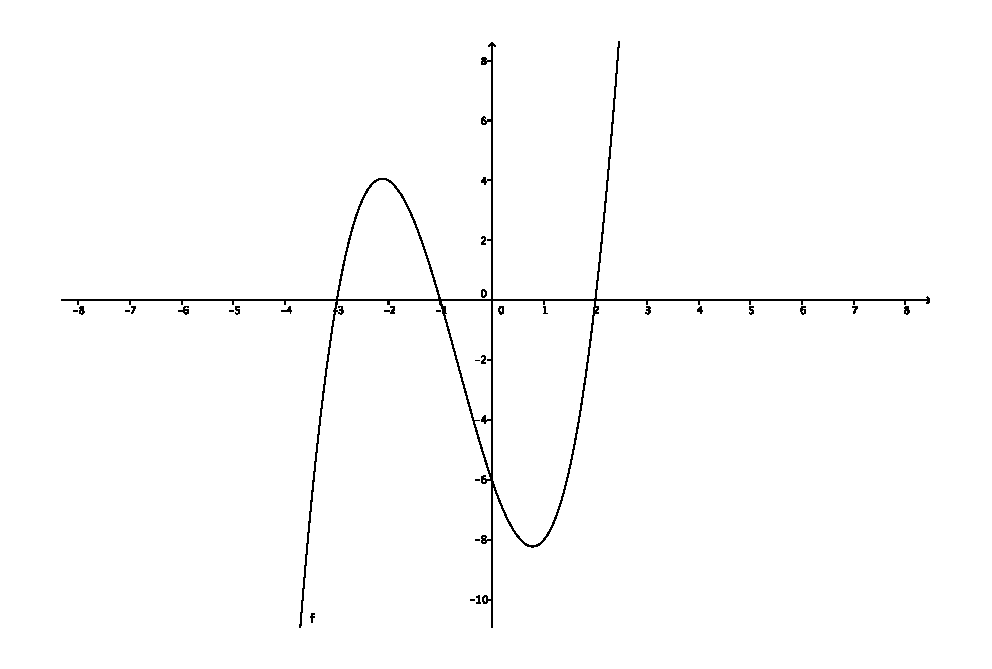
\includegraphics[width=6in]{Plot2A.pdf}
\end{center}


\end{enumerate}
\newpage

\item 
\begin{enumerate}
 \item Sketch the graph of $f(x) = \dfrac{x}{x^2-4}$. \points{6}

\bigskip

Since $f(x) = \dfrac{x}{(x-2)(x+2)}$, we see that $f(0)=0$ (so $(0,0)$ is both the $x$- and $y$-intercept), and the graph of $f$ has vertical asymptotes $x=2$ and $x=-2$. Since the degree of the denominator is less than the degree of the numerator, the graph $y=f(x)$ has $y=0$ as a horizontal asymptote. The sign diagram of $f$ is given by
\begin{center}
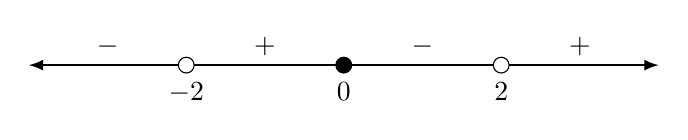
\begin{tikzpicture}[>=latex]
  \draw [thick, <->] (-4,0) -- (4,0);
  \draw [fill=white] (-2,0) circle [radius =.1];
  \draw [fill] (0,0) circle [radius =.1];
  \draw [fill=white] (2,0) circle [radius =.1];
  \node at (-3,0) [above] {$-$};
  \node at (-1,0) [above] {$+$};
  \node at (1,0) [above] {$-$};
  \node at (3,0) [above] {$+$};
  \node at (-2,-0.1) [below] {$-2$};
  \node at (0,-0.1) [below] {$0$};
  \node at (2,-0.1) [below] {$2$};
  \end{tikzpicture}
\end{center}
From the sign diagram we can determine the behaviour of $f(x)$ near the vertical asymptotes, giving us the graph
\begin{center}
 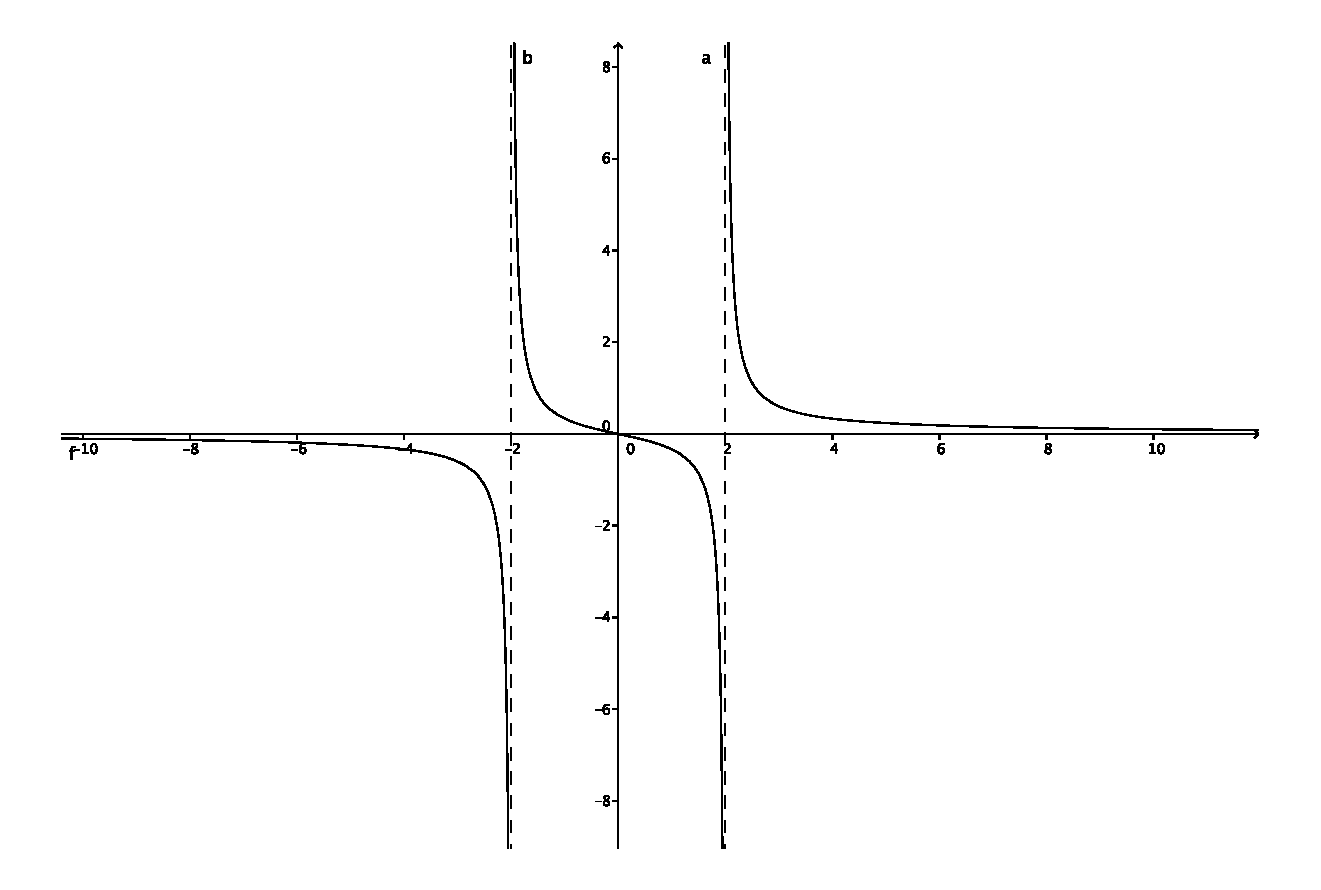
\includegraphics[width=4in]{Plot3A.pdf}
\end{center}

 \item Solve the rational inequality $\dfrac{6}{x-1}-\dfrac{6}{x}\geq 1$. \points{4} 

\bigskip

(Note: this problem was taken directly off one of your WeBWorK assignments.)

To solve the inequality, we move everything to the left-hand side and get a common denominator. We have
\begin{align*}
 \frac{6}{x-1}-\frac{6}{x}-1 &= \frac{6x-6(x-1)-1(x)(x-1)}{x(x-1)} = \frac{6x-6x+6-x^2+x}{x(x-1)}\\
& = \frac{-x^2+x+6}{x(x-1)} = \frac{-(x+2)(x-3)}{x(x-1)},
\end{align*}
so the original inequality is equivalent to $g(x)\geq 0$, where $g(x) = \dfrac{-(x+2)(x-3)}{x(x-1)}$. The sign diagram for $g(x)$ is:
\begin{center}
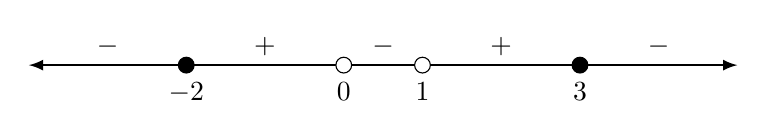
\begin{tikzpicture}[>=latex]
  \draw [thick, <->] (-4,0) -- (5,0);
  \draw [fill] (-2,0) circle [radius =.1];
  \draw [fill=white] (0,0) circle [radius =.1];
  \draw [fill=white] (1,0) circle [radius =.1];
  \draw [fill] (3,0) circle [radius =.1];
  \node at (-3,0) [above] {$-$};
  \node at (-1,0) [above] {$+$};
  \node at (0.5,0) [above] {$-$};
  \node at (2,0) [above] {$+$};
  \node at (4,0) [above] {$-$};
  \node at (-2,-0.1) [below] {$-2$};
  \node at (0,-0.1) [below] {$0$};
  \node at (1,-0.1) [below] {$1$};
  \node at (3,-0.1) [below] {$3$};
  \end{tikzpicture}
\end{center}
From the sign diagram, we see that $g(x)\geq 0$ for $x\in [-2,0)\cup (1,3]$.
\end{enumerate}

\newpage

\item \begin{enumerate}
       \item What are the values of $\cos\left(\dfrac{19\pi}{4}\right)$ and $\sin\left(\dfrac{-29\pi}{6}\right)$? \points{2}

\bigskip

Since $\dfrac{19\pi}{4} = \dfrac{16\pi}{4}+\dfrac{5\pi}{4} = 4\pi +\dfrac{5\pi}{4}$ is in Quadrant II, we have $\cos\left(\dfrac{19\pi}{4}\right) = -\dfrac{\sqrt{2}}{2}$.

\medskip

Since $-\dfrac{29\pi}{6} = -\dfrac{24\pi}{6}-\dfrac{5\pi}{6} = -4\pi - \dfrac{5\pi}{6}$ is in Quadrant III, we have $\sin\left(-\dfrac{29\pi}{6}\right) = -\dfrac{1}{2}$.

\bigskip

 \item What is the value of $\sin\left(\dfrac{5\pi}{12}\right)$? (Hint: $5=9-4$)\points{4}

\bigskip

Using the angle addition formula for $\sin$, we have
\begin{align*}
 \sin\left(\frac{5\pi}{12}\right) & = \sin\left(\frac{9\pi}{12}-\frac{4\pi}{12}\right) = \sin\left(\frac{3\pi}{4}-\frac{\pi}{3}\right)\\
& = \sin\left(\frac{3\pi}{4}\right)\cos\left(\frac{\pi}{4}\right)-\cos\left(\frac{3\pi}{4}\right)\sin\left(\frac{\pi}{3}\right)\\
& = \left(\frac{\sqrt{2}}{2}\right)\left(\frac{1}{2}\right) - \left(-\frac{\sqrt{2}}{2}\right)\left(\frac{\sqrt{3}}{2}\right) = \frac{\sqrt{2}+\sqrt{6}}{4}.
\end{align*}

\medskip

Alternatively, one can use the half-angle formula for $\sin$ to obtain
\[
 \sin\left(\frac{5\pi}{12}\right)  = \sin\left(\frac{1}{2}\cdot \frac{5\pi}{6}\right)\\
 = \sqrt{\frac{1-\cos(5\pi/6)}{2}} = \sqrt{\frac{1+\sqrt{3}/2}{2}} = \sqrt{\frac{2+\sqrt{3}}{4}}.
\]

\bigskip



\item Verify the identity $\dfrac{1}{1-\sin\theta} = \sec^2\theta+\sec\theta\tan\theta$. \points{4}

\bigskip

Beginning with the right-hand side (and taking care not to set the two sides equal to each other before we've verified that they are, in fact, equal), we have
\begin{align*}
 \sec^2\theta+\sec\theta\tan\theta & = \frac{1}{\cos^2\theta}+\frac{1}{\cos\theta}\left(\frac{\sin\theta}{\cos\theta}\right)\\
& = \frac{1}{\cos^2\theta}+\frac{\sin\theta}{\cos^2\theta}\\
& = \frac{1+\sin\theta}{\cos^2\theta}\\
& = \frac{1+\sin\theta}{1-\sin^2\theta}\\
& = \frac{1+\sin\theta}{(1+\sin\theta)(1-\sin\theta)}\\
& = \frac{1}{1-\sin\theta},
\end{align*}
giving us the left-hand side.
      \end{enumerate}


\end{enumerate}

\end{document}